% Created by tikzDevice version 0.12
% !TEX encoding = UTF-8 Unicode
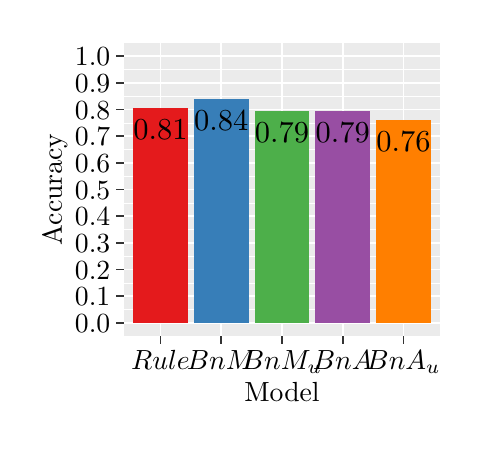
\begin{tikzpicture}[x=1pt,y=1pt]
\definecolor{fillColor}{RGB}{255,255,255}
\path[use as bounding box,fill=fillColor,fill opacity=0.00] (0,0) rectangle (154.47,142.39);
\begin{scope}
\path[clip] (  0.00,  0.00) rectangle (154.47,142.39);
\definecolor{drawColor}{RGB}{255,255,255}
\definecolor{fillColor}{RGB}{255,255,255}

\path[draw=drawColor,line width= 0.6pt,line join=round,line cap=round,fill=fillColor] (  0.00,  0.00) rectangle (154.47,142.39);
\end{scope}
\begin{scope}
\path[clip] ( 34.81, 30.86) rectangle (148.97,136.89);
\definecolor{fillColor}{gray}{0.92}

\path[fill=fillColor] ( 34.81, 30.86) rectangle (148.97,136.89);
\definecolor{drawColor}{RGB}{255,255,255}

\path[draw=drawColor,line width= 0.3pt,line join=round] ( 34.81, 40.50) --
	(148.97, 40.50);

\path[draw=drawColor,line width= 0.3pt,line join=round] ( 34.81, 50.14) --
	(148.97, 50.14);

\path[draw=drawColor,line width= 0.3pt,line join=round] ( 34.81, 59.78) --
	(148.97, 59.78);

\path[draw=drawColor,line width= 0.3pt,line join=round] ( 34.81, 69.42) --
	(148.97, 69.42);

\path[draw=drawColor,line width= 0.3pt,line join=round] ( 34.81, 79.06) --
	(148.97, 79.06);

\path[draw=drawColor,line width= 0.3pt,line join=round] ( 34.81, 88.69) --
	(148.97, 88.69);

\path[draw=drawColor,line width= 0.3pt,line join=round] ( 34.81, 98.33) --
	(148.97, 98.33);

\path[draw=drawColor,line width= 0.3pt,line join=round] ( 34.81,107.97) --
	(148.97,107.97);

\path[draw=drawColor,line width= 0.3pt,line join=round] ( 34.81,117.61) --
	(148.97,117.61);

\path[draw=drawColor,line width= 0.3pt,line join=round] ( 34.81,127.25) --
	(148.97,127.25);

\path[draw=drawColor,line width= 0.6pt,line join=round] ( 34.81, 35.68) --
	(148.97, 35.68);

\path[draw=drawColor,line width= 0.6pt,line join=round] ( 34.81, 45.32) --
	(148.97, 45.32);

\path[draw=drawColor,line width= 0.6pt,line join=round] ( 34.81, 54.96) --
	(148.97, 54.96);

\path[draw=drawColor,line width= 0.6pt,line join=round] ( 34.81, 64.60) --
	(148.97, 64.60);

\path[draw=drawColor,line width= 0.6pt,line join=round] ( 34.81, 74.24) --
	(148.97, 74.24);

\path[draw=drawColor,line width= 0.6pt,line join=round] ( 34.81, 83.87) --
	(148.97, 83.87);

\path[draw=drawColor,line width= 0.6pt,line join=round] ( 34.81, 93.51) --
	(148.97, 93.51);

\path[draw=drawColor,line width= 0.6pt,line join=round] ( 34.81,103.15) --
	(148.97,103.15);

\path[draw=drawColor,line width= 0.6pt,line join=round] ( 34.81,112.79) --
	(148.97,112.79);

\path[draw=drawColor,line width= 0.6pt,line join=round] ( 34.81,122.43) --
	(148.97,122.43);

\path[draw=drawColor,line width= 0.6pt,line join=round] ( 34.81,132.07) --
	(148.97,132.07);

\path[draw=drawColor,line width= 0.6pt,line join=round] ( 47.98, 30.86) --
	( 47.98,136.89);

\path[draw=drawColor,line width= 0.6pt,line join=round] ( 69.93, 30.86) --
	( 69.93,136.89);

\path[draw=drawColor,line width= 0.6pt,line join=round] ( 91.89, 30.86) --
	( 91.89,136.89);

\path[draw=drawColor,line width= 0.6pt,line join=round] (113.84, 30.86) --
	(113.84,136.89);

\path[draw=drawColor,line width= 0.6pt,line join=round] (135.80, 30.86) --
	(135.80,136.89);
\definecolor{fillColor}{RGB}{228,26,28}

\path[fill=fillColor] ( 38.10, 35.68) rectangle ( 57.86,113.53);
\definecolor{fillColor}{RGB}{55,126,184}

\path[fill=fillColor] ( 60.05, 35.68) rectangle ( 79.81,116.60);
\definecolor{fillColor}{RGB}{77,175,74}

\path[fill=fillColor] ( 82.01, 35.68) rectangle (101.77,112.23);
\definecolor{fillColor}{RGB}{152,78,163}

\path[fill=fillColor] (103.96, 35.68) rectangle (123.72,112.29);
\definecolor{fillColor}{RGB}{255,127,0}

\path[fill=fillColor] (125.92, 35.68) rectangle (145.68,109.02);
\definecolor{drawColor}{RGB}{0,0,0}

\node[text=drawColor,anchor=base,inner sep=0pt, outer sep=0pt, scale=  1.10] at (135.80, 97.61) {0.76};

\node[text=drawColor,anchor=base,inner sep=0pt, outer sep=0pt, scale=  1.10] at (113.84,100.89) {0.79};

\node[text=drawColor,anchor=base,inner sep=0pt, outer sep=0pt, scale=  1.10] at ( 91.89,100.83) {0.79};

\node[text=drawColor,anchor=base,inner sep=0pt, outer sep=0pt, scale=  1.10] at ( 69.93,105.19) {0.84};

\node[text=drawColor,anchor=base,inner sep=0pt, outer sep=0pt, scale=  1.10] at ( 47.98,102.12) {0.81};
\end{scope}
\begin{scope}
\path[clip] (  0.00,  0.00) rectangle (154.47,142.39);
\definecolor{drawColor}{RGB}{0,0,0}

\node[text=drawColor,anchor=base east,inner sep=0pt, outer sep=0pt, scale=  1.00] at ( 29.86, 32.24) {0.0};

\node[text=drawColor,anchor=base east,inner sep=0pt, outer sep=0pt, scale=  1.00] at ( 29.86, 41.88) {0.1};

\node[text=drawColor,anchor=base east,inner sep=0pt, outer sep=0pt, scale=  1.00] at ( 29.86, 51.52) {0.2};

\node[text=drawColor,anchor=base east,inner sep=0pt, outer sep=0pt, scale=  1.00] at ( 29.86, 61.15) {0.3};

\node[text=drawColor,anchor=base east,inner sep=0pt, outer sep=0pt, scale=  1.00] at ( 29.86, 70.79) {0.4};

\node[text=drawColor,anchor=base east,inner sep=0pt, outer sep=0pt, scale=  1.00] at ( 29.86, 80.43) {0.5};

\node[text=drawColor,anchor=base east,inner sep=0pt, outer sep=0pt, scale=  1.00] at ( 29.86, 90.07) {0.6};

\node[text=drawColor,anchor=base east,inner sep=0pt, outer sep=0pt, scale=  1.00] at ( 29.86, 99.71) {0.7};

\node[text=drawColor,anchor=base east,inner sep=0pt, outer sep=0pt, scale=  1.00] at ( 29.86,109.35) {0.8};

\node[text=drawColor,anchor=base east,inner sep=0pt, outer sep=0pt, scale=  1.00] at ( 29.86,118.99) {0.9};

\node[text=drawColor,anchor=base east,inner sep=0pt, outer sep=0pt, scale=  1.00] at ( 29.86,128.62) {1.0};
\end{scope}
\begin{scope}
\path[clip] (  0.00,  0.00) rectangle (154.47,142.39);
\definecolor{drawColor}{gray}{0.20}

\path[draw=drawColor,line width= 0.6pt,line join=round] ( 32.06, 35.68) --
	( 34.81, 35.68);

\path[draw=drawColor,line width= 0.6pt,line join=round] ( 32.06, 45.32) --
	( 34.81, 45.32);

\path[draw=drawColor,line width= 0.6pt,line join=round] ( 32.06, 54.96) --
	( 34.81, 54.96);

\path[draw=drawColor,line width= 0.6pt,line join=round] ( 32.06, 64.60) --
	( 34.81, 64.60);

\path[draw=drawColor,line width= 0.6pt,line join=round] ( 32.06, 74.24) --
	( 34.81, 74.24);

\path[draw=drawColor,line width= 0.6pt,line join=round] ( 32.06, 83.87) --
	( 34.81, 83.87);

\path[draw=drawColor,line width= 0.6pt,line join=round] ( 32.06, 93.51) --
	( 34.81, 93.51);

\path[draw=drawColor,line width= 0.6pt,line join=round] ( 32.06,103.15) --
	( 34.81,103.15);

\path[draw=drawColor,line width= 0.6pt,line join=round] ( 32.06,112.79) --
	( 34.81,112.79);

\path[draw=drawColor,line width= 0.6pt,line join=round] ( 32.06,122.43) --
	( 34.81,122.43);

\path[draw=drawColor,line width= 0.6pt,line join=round] ( 32.06,132.07) --
	( 34.81,132.07);
\end{scope}
\begin{scope}
\path[clip] (  0.00,  0.00) rectangle (154.47,142.39);
\definecolor{drawColor}{gray}{0.20}

\path[draw=drawColor,line width= 0.6pt,line join=round] ( 47.98, 28.11) --
	( 47.98, 30.86);

\path[draw=drawColor,line width= 0.6pt,line join=round] ( 69.93, 28.11) --
	( 69.93, 30.86);

\path[draw=drawColor,line width= 0.6pt,line join=round] ( 91.89, 28.11) --
	( 91.89, 30.86);

\path[draw=drawColor,line width= 0.6pt,line join=round] (113.84, 28.11) --
	(113.84, 30.86);

\path[draw=drawColor,line width= 0.6pt,line join=round] (135.80, 28.11) --
	(135.80, 30.86);
\end{scope}
\begin{scope}
\path[clip] (  0.00,  0.00) rectangle (154.47,142.39);
\definecolor{drawColor}{RGB}{0,0,0}

\node[text=drawColor,anchor=base,inner sep=0pt, outer sep=0pt, scale=  1.00] at ( 47.98, 19.03) {\(Rule\)};

\node[text=drawColor,anchor=base,inner sep=0pt, outer sep=0pt, scale=  1.00] at ( 69.93, 19.03) {\(BnM\)};

\node[text=drawColor,anchor=base,inner sep=0pt, outer sep=0pt, scale=  1.00] at ( 91.89, 19.03) {\(BnM_u\)};

\node[text=drawColor,anchor=base,inner sep=0pt, outer sep=0pt, scale=  1.00] at (113.84, 19.03) {\(BnA\)};

\node[text=drawColor,anchor=base,inner sep=0pt, outer sep=0pt, scale=  1.00] at (135.80, 19.03) {\(BnA_u\)};
\end{scope}
\begin{scope}
\path[clip] (  0.00,  0.00) rectangle (154.47,142.39);
\definecolor{drawColor}{RGB}{0,0,0}

\node[text=drawColor,anchor=base,inner sep=0pt, outer sep=0pt, scale=  1.00] at ( 91.89,  7.44) {Model};
\end{scope}
\begin{scope}
\path[clip] (  0.00,  0.00) rectangle (154.47,142.39);
\definecolor{drawColor}{RGB}{0,0,0}

\node[text=drawColor,rotate= 90.00,anchor=base,inner sep=0pt, outer sep=0pt, scale=  1.00] at ( 12.39, 83.87) {Accuracy};
\end{scope}
\end{tikzpicture}
